\documentclass[11pt]{article}
\usepackage[utf8]{inputenc}
\usepackage{titling}
\usepackage{graphicx}
\usepackage{amsmath}
\usepackage{amssymb}
\usepackage{color}
\usepackage{float}
\usepackage{gensymb}
\usepackage[english]{babel}
\usepackage{tabularx}
\usepackage{geometry}
\usepackage[parfill]{parskip}
\usepackage{mathrsfs}
\usepackage{hyperref}
%\usepackage{subcaption}
\usepackage{multicol}
\usepackage{dirtytalk}
\usepackage{subfig}
\setlength{\columnsep}{.8cm}
\geometry{a4paper,
 total={210mm,297mm},
 left=33mm,
 right=33mm,
 top=30mm,
 bottom=30mm,}
\newcommand{\code}[1]{{\texttt{#1}}}
\usepackage{titlesec}
\title{\huge IBM Minsky project proposal}

\author{Eric Wulff}
\date{\today}

\begin{document}

\maketitle

\section{Background and motivation}


Storage is one of the main limiting factor to the recording of information from proton-proton collisions events at the Large Hadron Collider, at CERN in Geneva. Hence, ATLAS uses a so called "trigger system", which selects and sends interesting events to the data storage system while throwing away the rest. However, if interesting events are buried in very large backgrounds and difficult to identify as signal by the trigger system, they will also be discarded together with the background. To overcome this problem, we plan to study compression algorithms that can be used directly by the trigger system. A variety of compression algorithms is already in use in high energy physics (see e.g. Ref.  https://iopscience.iop.org/article/10.1088/1742-6596/898/7/072043/pdf). 

In this project we plan to prototype data compression at the trigger level using autoencoder networks, where the smaller "hidden layer" of an auto encoder is retained and then decoded at a later stage. This is part of a Master's thesis project in collaboration between LTH and the ATLAS group in the particle physics division of the Natural Sciences Physics department at Lund University, under the supervision of Caterina Doglioni. This project is co-supervised by Lukas Heinrich (CERN) and Antonio Boveia (Ohio State University).  


Current technological limitations make it impossible to store the enormous amount of data that gets produced in high energy physics particle detectors. Hence, ATLAS uses a so called \emph{trigger system}~\cite{trigger_das}, consisting of two levels, one hardware level and one software level. The trigger system selects and sends interesting events to a data storage system while disregarding the rest.

This data reduction impairs the potential of discovering new particles that are buried in high-rate backgrounds. Therefore, a new technique called "Trigger Level Analysis" (TLA) has been brought forward by the Lund and OSU groups among others, to only record high-level information necessary to perform searches for those new particles. Since the size of each event is smaller, more events can be recorded, as shown in Fig.~\ref{TLA}. 

\begin{figure}[H]
\centering
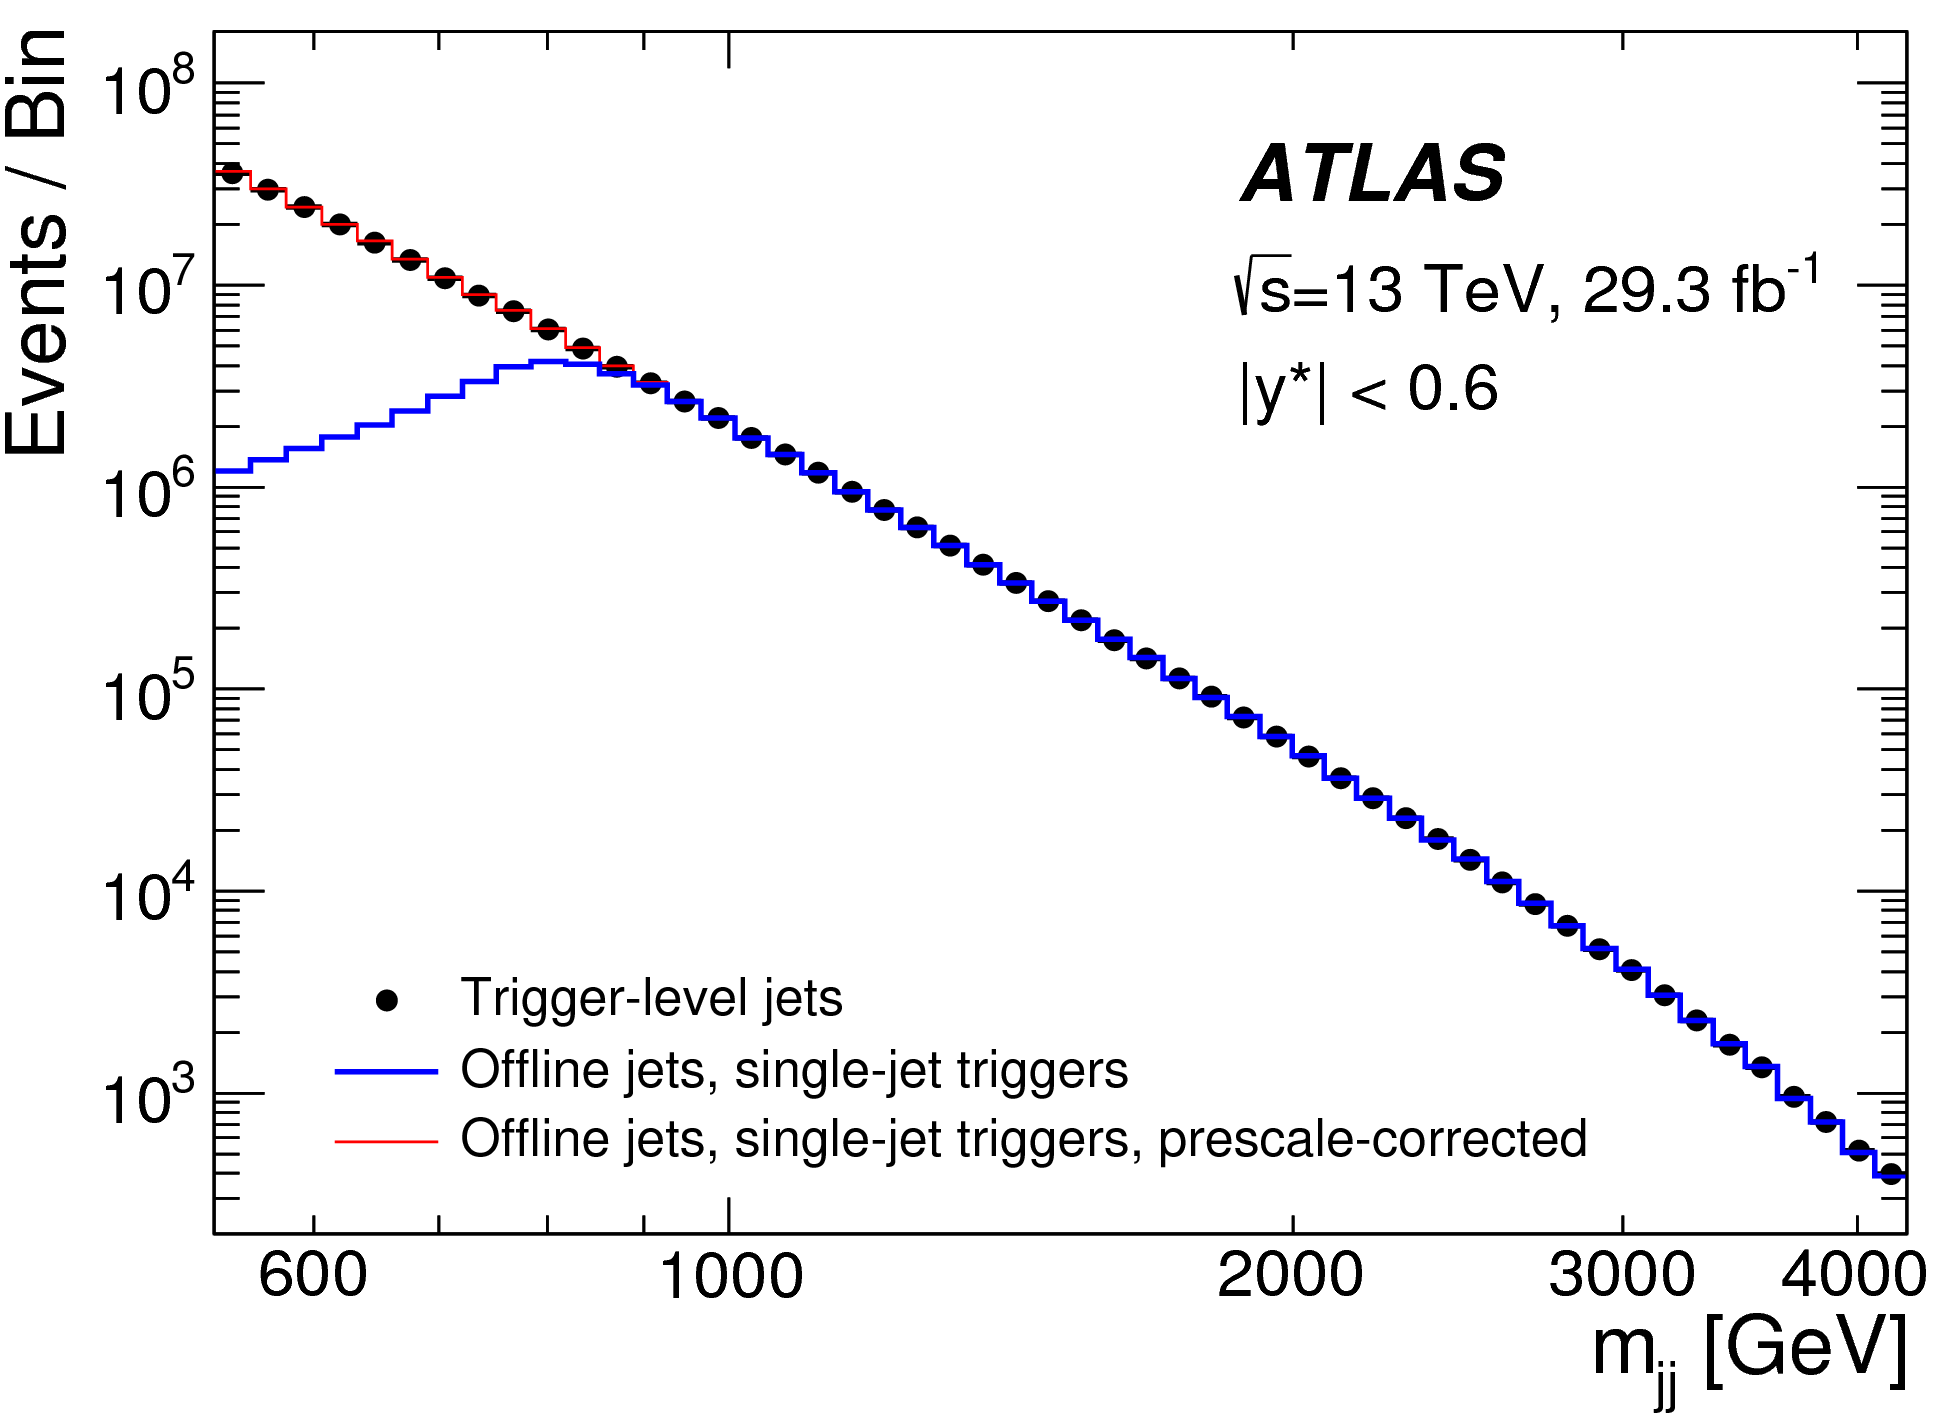
\includegraphics[width=0.6\textwidth]{TLA.png}
\caption{Improvement in number of events recorded with the TLA technique (black) with respect to the standard data taking techniques (blue line).}
\label{TLA}
\end{figure}

A further reduction of the current event size will allow us to perform searches that were not previously possible, for example for even lower mass dark matter mediators~\cite{Chala2015}. 

The focus of this project is to understand whether it is possible to further reduce the size of previously mentioned collision events using machine learning (ML) techniques for data compression and to compare the performance of these techniques with standard compression methods. This has never been tried before within the ATLAS experiment and it is an interesting forward-looking study for future experiments. Furthermore, a byproduct of this project is that we will gain expertise in cutting-edge machine learning techniques, and learn to use them in the context of both data compression and detection of anomalous events. 

It will also be interesting to treat this study as a proof-of-principle for future data compression techniques for the ATLAS experiment. For the planned experimental upgrades in 2026, the techniques used in this report may help solving the problem of needing much more storage space than in the past due to the increase of the size of the dataset, as shown in Fig~\ref{diskHLLHC}.

\begin{figure}[H]
\centering
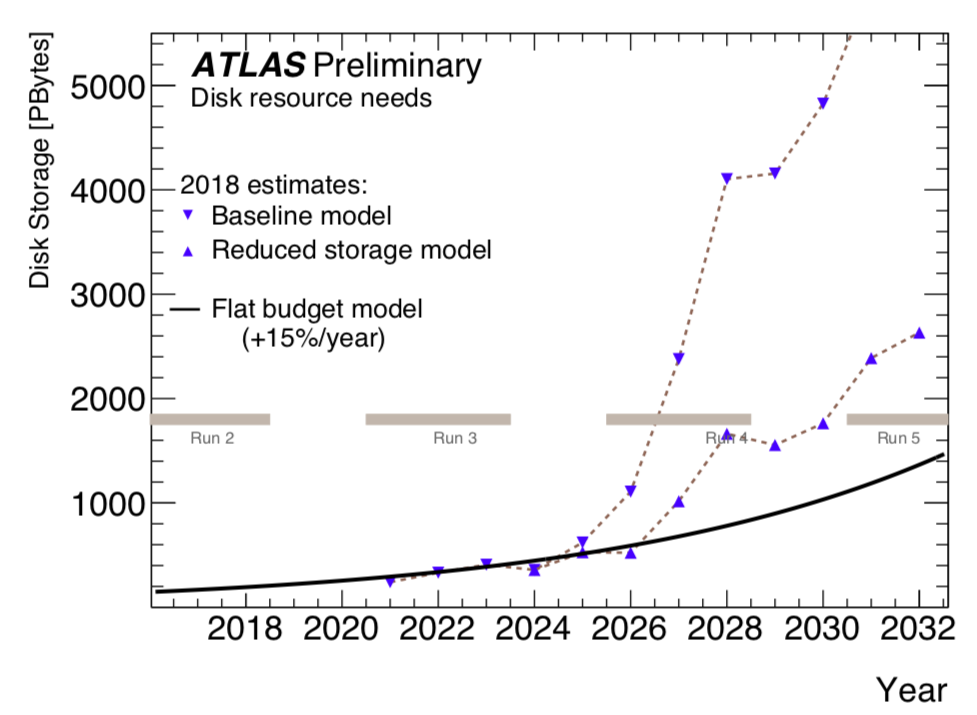
\includegraphics[width=0.6\textwidth]{diskHLLHC_noold.png}
\caption{Estimated future disk space required for storage of experimental data captured by ATLAS.}
\label{diskHLLHC}
\end{figure}


\section{Project outline}

This project will be carried out by Eric Wulff in his pursuit of a degree in Master of Science in Engineering (MSE) at Lund University under the supervision of Caterina Doglioni, Antonio Boveia and Lukas Heinrich. Upon the completion of the project in January 2020 the resulting thesis will be published in the Lund University library system, which is open to the public.

A machine learning (ML) approach will be used to complete the objective, specifically a method using autoencoder (AE) neural networks. In short an AE is a neural network which tries to implement an approximation to the identity, $f(x) \approx x$, by using one or more hidden layers with smaller size than the input and output layers. If this is possible, it means that all the information necessary to reproduce the input, $x$, is contained in the hidden layer, and the data has been compressed. The idea is then to only save this smaller hidden layer representation instead of the current data format, along with the neural network that can recreate the original data. 

Moreover, an AE can be used for anomaly detection. This is perhaps the most common use of AEs and works as follows. The AE is first trained on data which is known not to be anomalous. If then the network is presented with a new data point that differs in some significant way from the training data, the AE will not be able to provide a faithful reconstruction at the output layer and hence the data point is considered anomalous. In other words, if the \emph{reconstruction error} of a data point is larger than some threshold, it is considered anomalous.

Prototyping of simple AE architectures has already begun and some progress have been made. Figs.~\ref{fig:ae_200_hists}, \ref{fig:ae_200_residuals} and~\ref{fig:ae_200_plots} show results from a first attempt at compressing 4 dimensional representations of jets into 3 dimensions using a 3D latent space AE. In order to further explore more exotic architectures and to perform hyperparameter scans, the need fore computing power is a limiting factor. IBM's Minsky platform provides access to powerful compute nodes with GPUs suited for training deep neural networks. Furthermore, they provide tools for easily doing hyperparameter scans. This would be very helpful to this project and could greatly increase the potential progress that can be made within the its set time period.

%\begin{figure}[H]
%\subfloat[Transverse momentum]{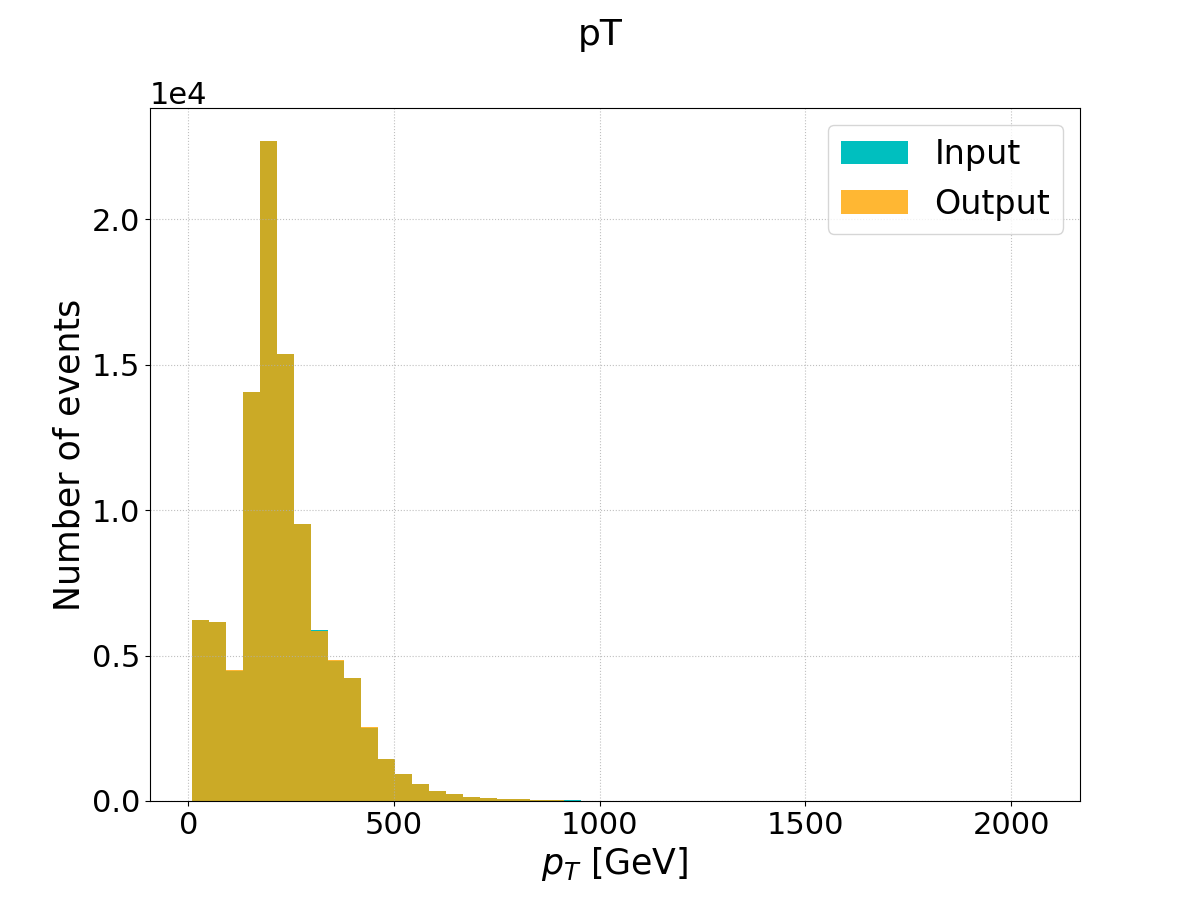
\includegraphics[trim={0.0cm 0.0cm 0.0cm 1.4cm},clip,width=0.5\textwidth]{figures/AE_3D_v2_hist_pT.png}} 
%\subfloat[Pseudorapidity]{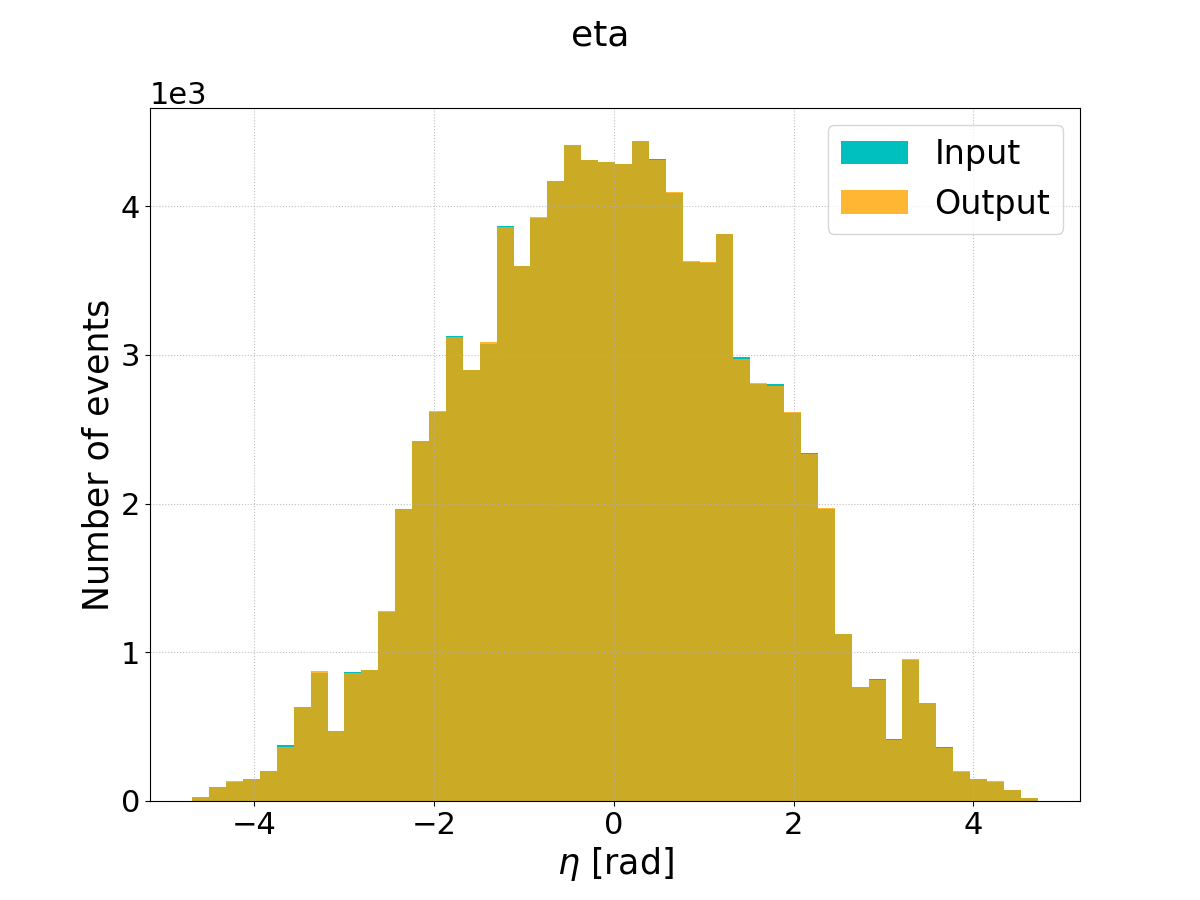
\includegraphics[trim={0.0cm 0.0cm 0.0cm 1.4cm},clip,width=0.5\textwidth]{figures/AE_3D_v2_hist_eta.png}}\\
%\subfloat[Azimuthal angle]{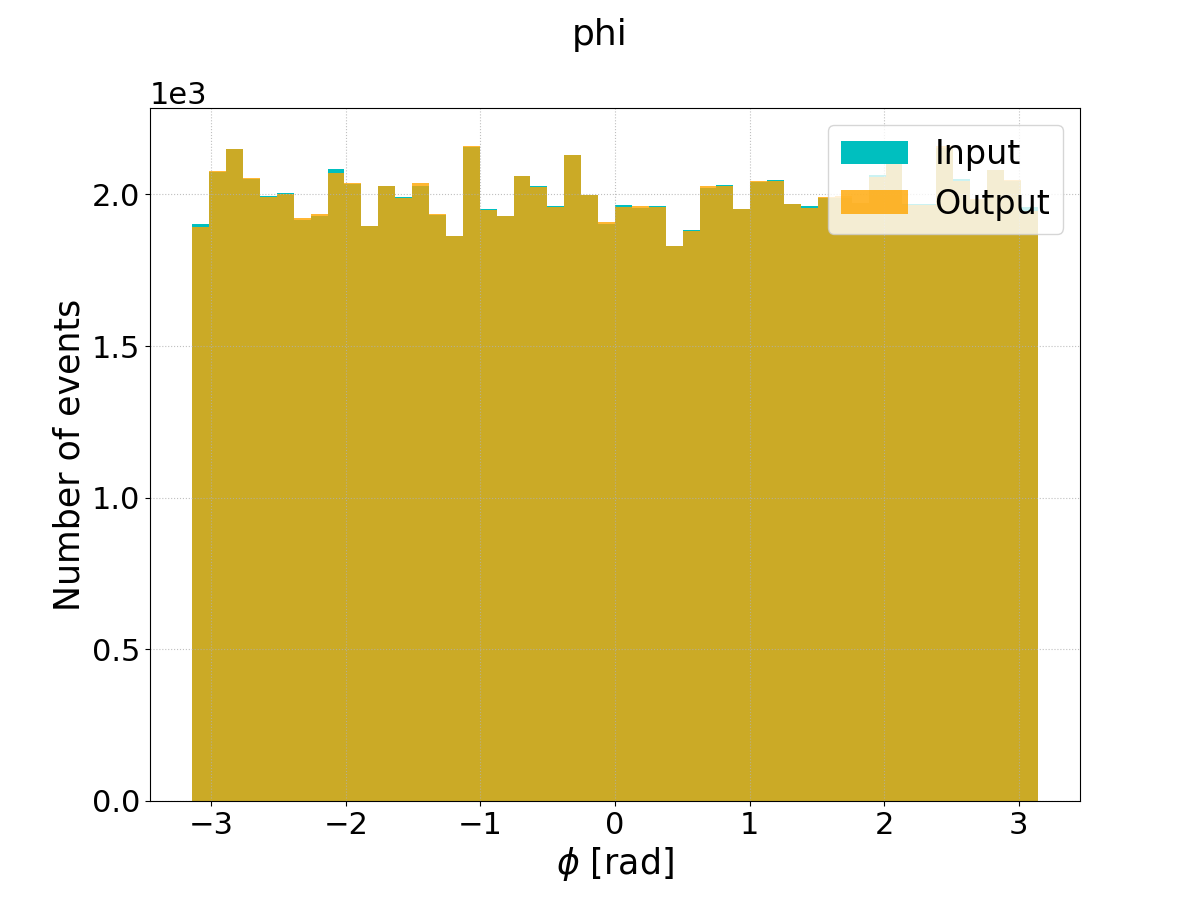
\includegraphics[trim={0.0cm 0.0cm 0.0cm 1.4cm},clip,width=0.5\textwidth]{figures/AE_3D_v2_hist_phi.png}}
%\subfloat[Energy]{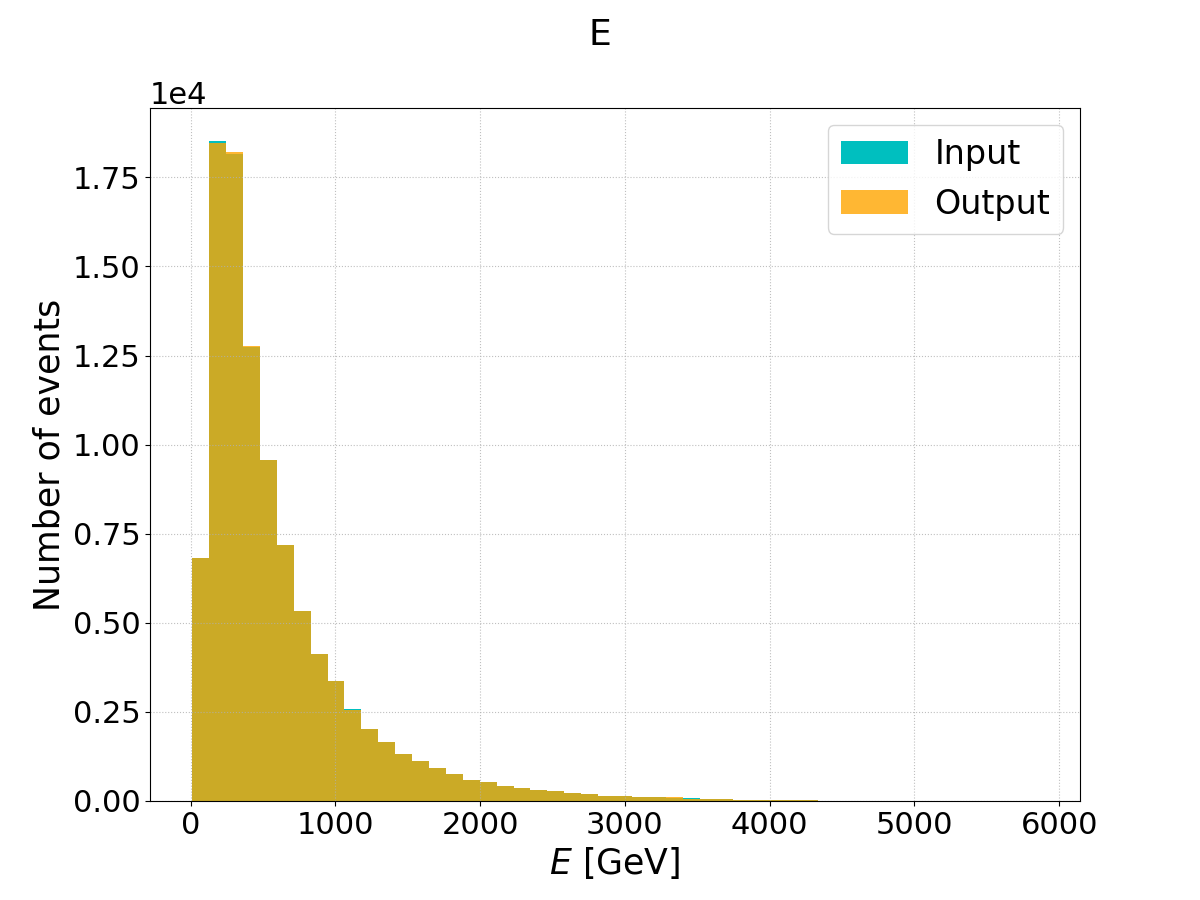
\includegraphics[trim={0.0cm 0.0cm 0.0cm 1.4cm},clip,width=0.5\textwidth]{figures/AE_3D_v2_hist_E.png}} 
%\caption{Histograms comparing the input and output of a prototyped AE with seven hidden layers and \{200, 100, 50, 3, 50, 100, 200\} nodes in each layer. The AE was trained on $~1.55 \cdot 10^6$ jets. The histograms shown here are produced from a validation set containing $~3.4 \cdot 10^5$ jets.} 
%\label{fig:ae_200_hists}
%\end{figure}

\begin{figure}[H]
\subfloat[Residuals of the transverse momentum]{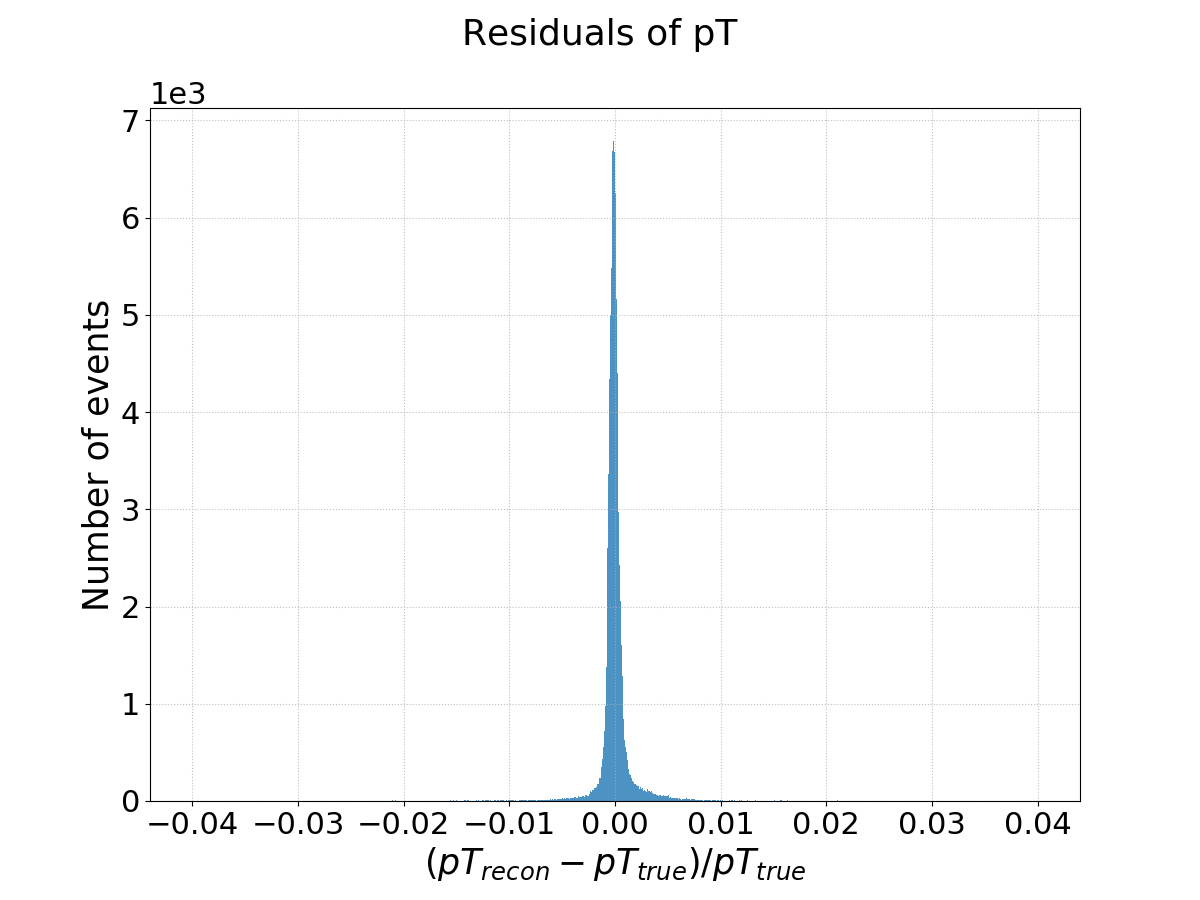
\includegraphics[trim={0.0cm 0.0cm 0.0cm 1.4cm},clip,width=0.5\textwidth]{figures/AE_3D_v2_residuals_pT.png}} 
\subfloat[Residuals of the pseudorapidity]{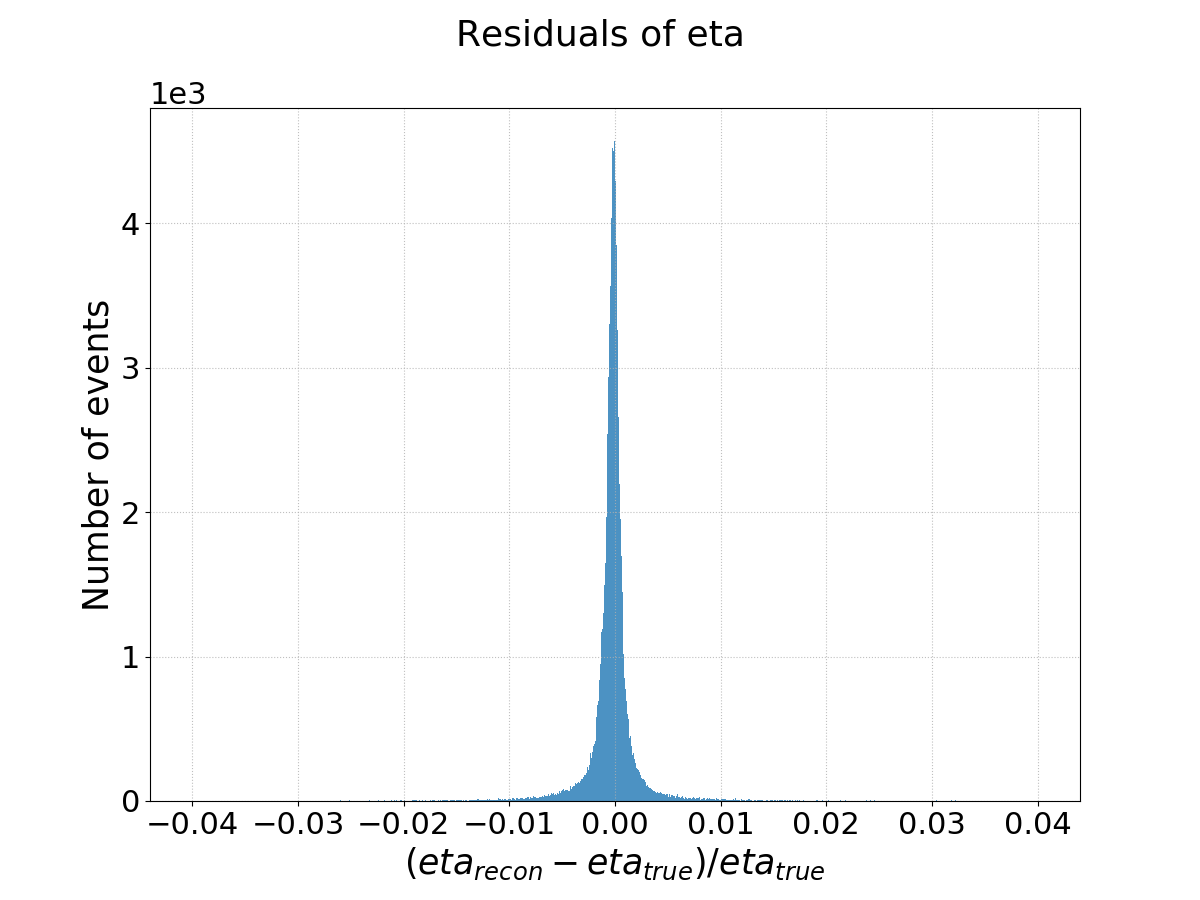
\includegraphics[trim={0.0cm 0.0cm 0.0cm 1.4cm},clip,width=0.5\textwidth]{figures/AE_3D_v2_residuals_eta.png}}\\
\subfloat[Residuals of the azimuthal angle]{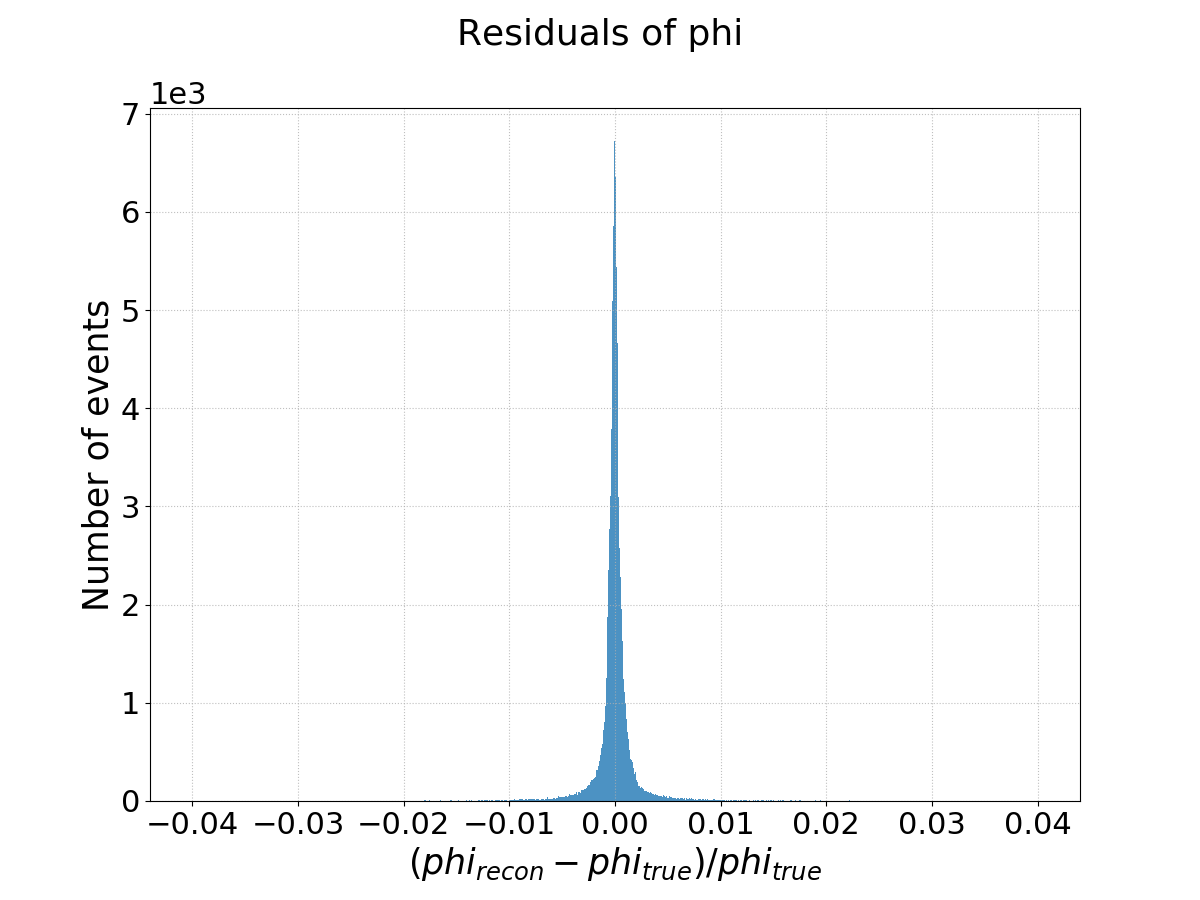
\includegraphics[trim={0.0cm 0.0cm 0.0cm 1.4cm},clip,width=0.5\textwidth]{figures/AE_3D_v2_residuals_phi.png}}
\subfloat[Residuals of the energy]{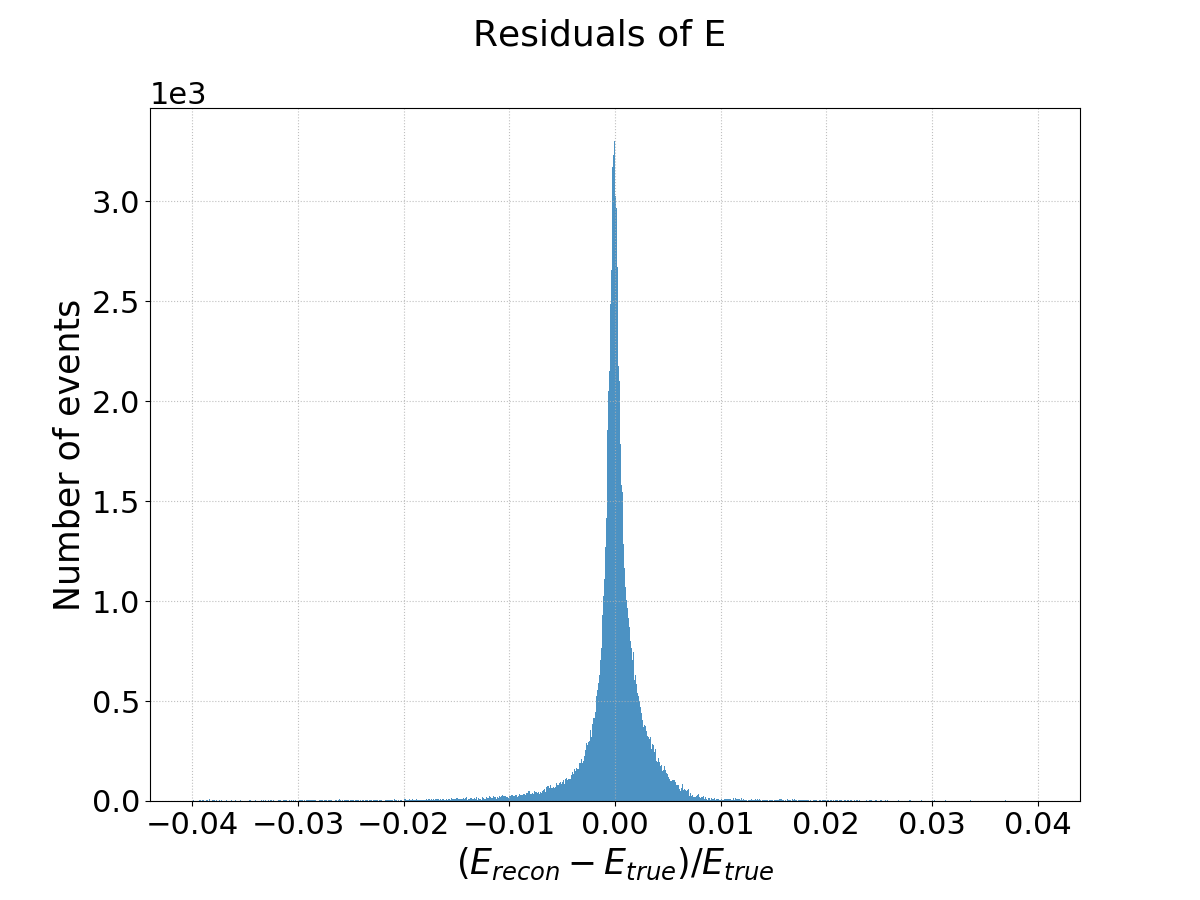
\includegraphics[trim={0.0cm 0.0cm 0.0cm 1.4cm},clip,width=0.5\textwidth]{figures/AE_3D_v2_residuals_E.png}} 
\caption{Histograms of the residuals of the input and output shown in Fig.~\ref{fig:ae_200_hists}. Almost all residuals are smaller than 1\%.} 
\label{fig:ae_200_residuals}
\end{figure}


\begin{figure}[H]
\subfloat[Residuals of the transverse momentum]{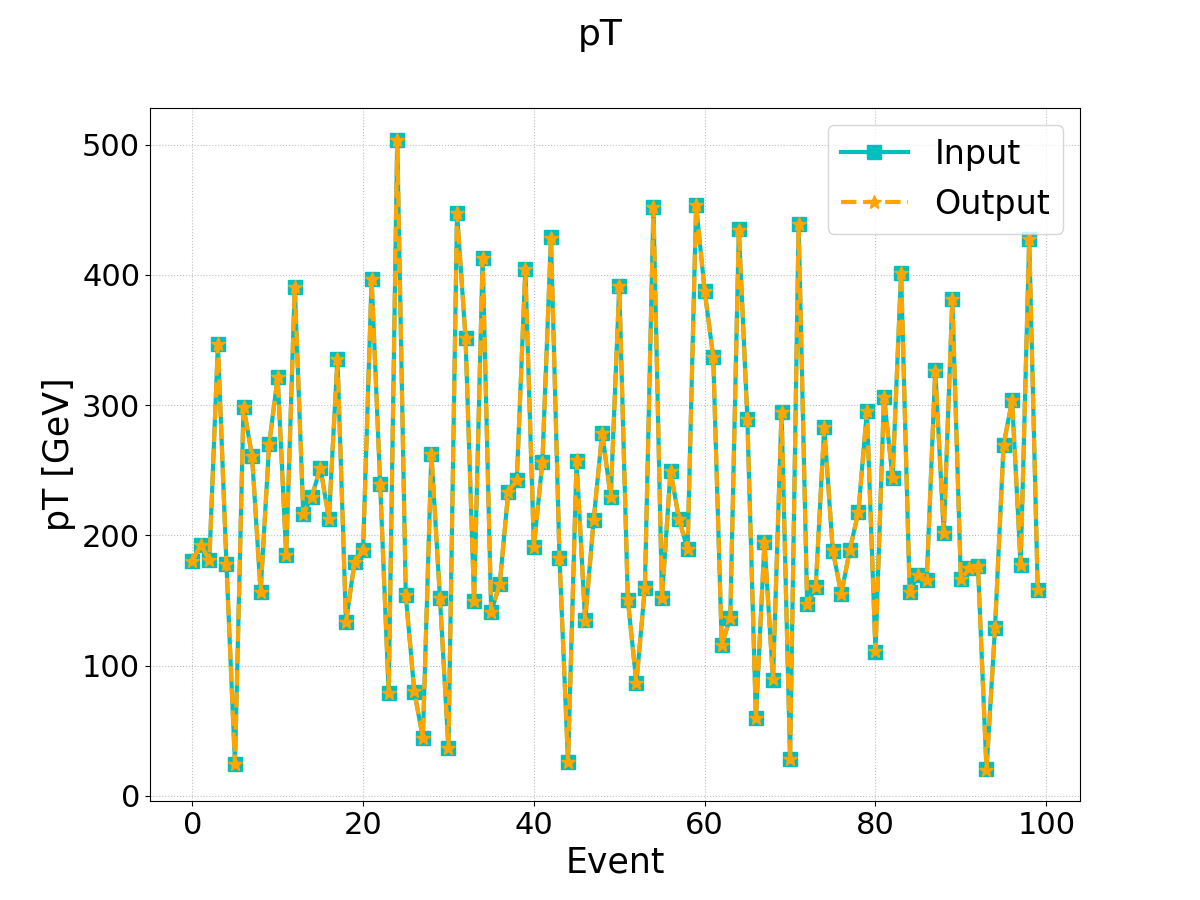
\includegraphics[trim={0.0cm 0.0cm 0.0cm 1.4cm},clip,width=0.5\textwidth]{figures/AE_3D_v2_plot_pT.png}} 
\subfloat[Residuals of the pseudorapidity]{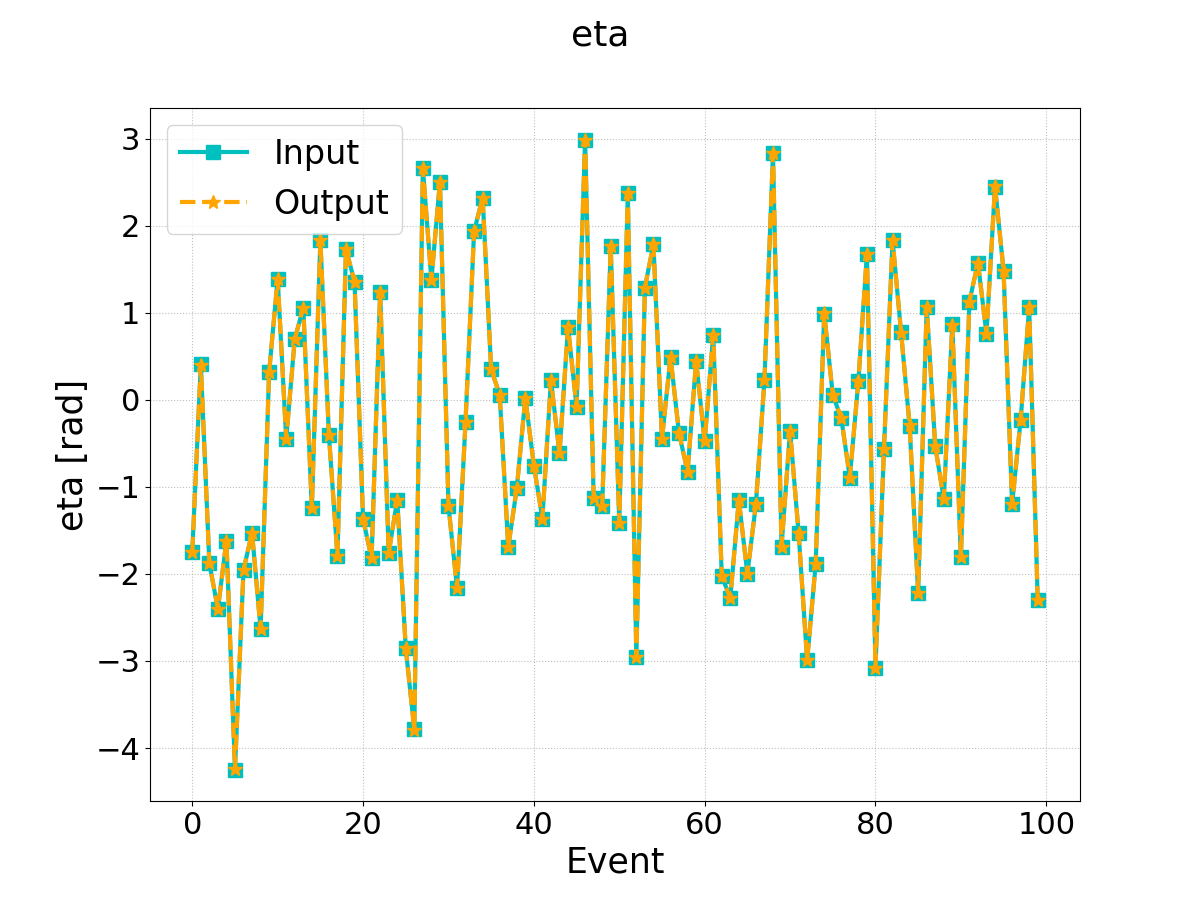
\includegraphics[trim={0.0cm 0.0cm 0.0cm 1.4cm},clip,width=0.5\textwidth]{figures/AE_3D_v2_plot_eta.png}}\\
\subfloat[Residuals of the azimuthal angle]{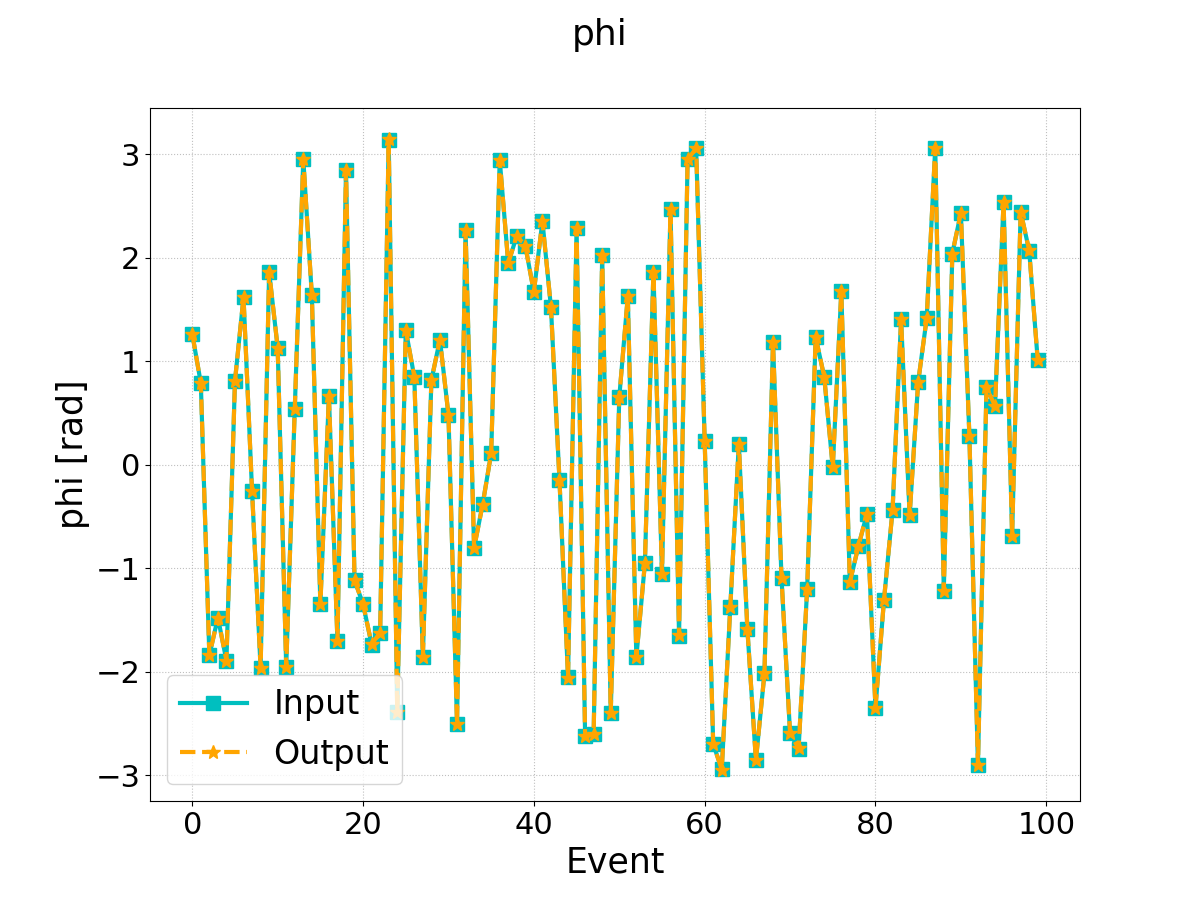
\includegraphics[trim={0.0cm 0.0cm 0.0cm 1.4cm},clip,width=0.5\textwidth]{figures/AE_3D_v2_plot_phi.png}}
\subfloat[Residuals of the energy]{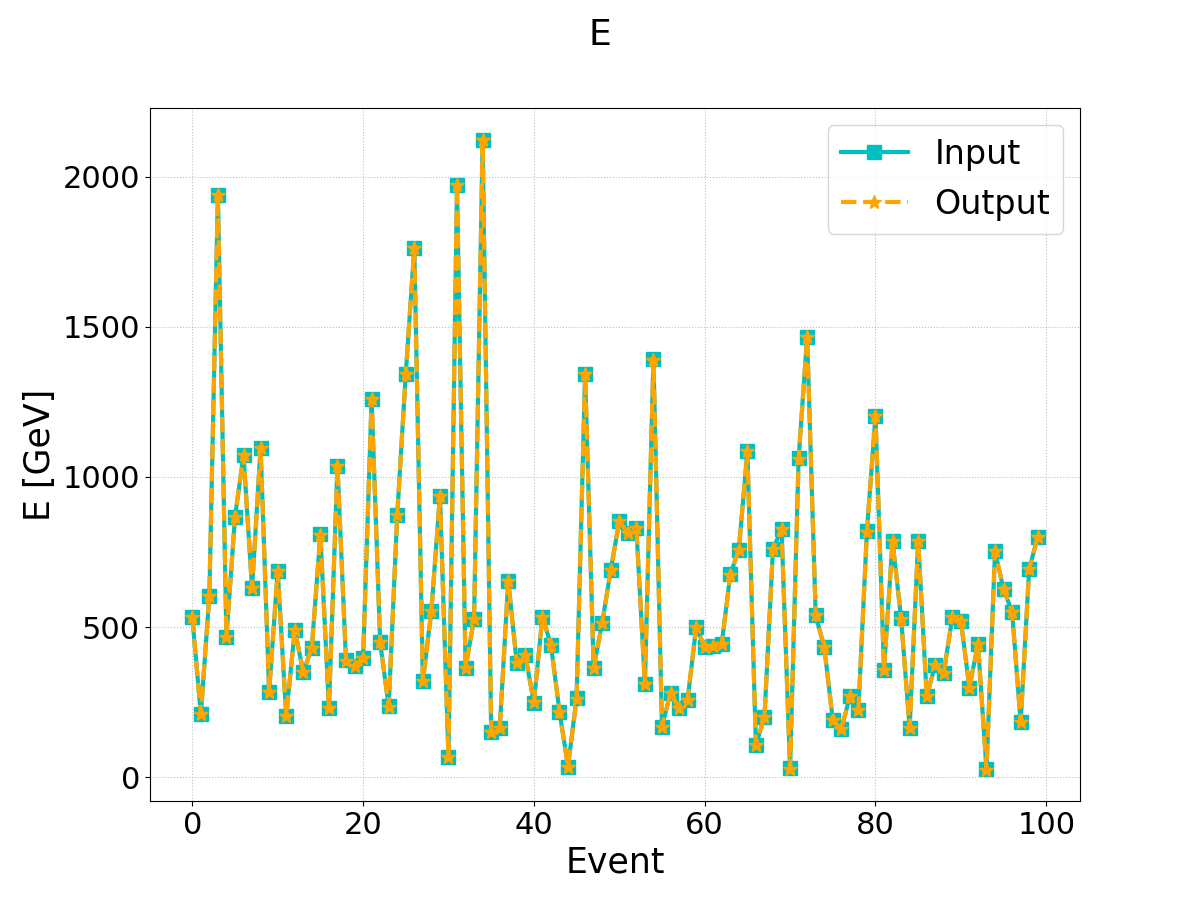
\includegraphics[trim={0.0cm 0.0cm 0.0cm 1.4cm},clip,width=0.5\textwidth]{figures/AE_3D_v2_plot_E.png}} 
\caption{Comparison of the input and output of a prototyped AE with seven hidden layers and \{200, 100, 50, 3, 50, 100, 200\} nodes in each layer. The AE was trained on $~1.55 \cdot 10^6$ jets.  Here the comparison of input and output of the AE uses only the leading jets from 100 events.
The histograms shown here are produced %from a validation set containing $~3.4 \cdot 10^5$ jets.
}
\label{fig:ae_200_plots}
\end{figure}


\section{Project Milestones}

\begin{itemize}
    \item Build and train an AE to compress physics events jet-by-jet
    \item Do an exploratory analysis of different AE architectures
    \item Perform computing intensive hyperparameter scans
    \item Build and train an AE to compress full events
    \item Compare and benchmark the achieved compression of the AEs with existing ATLAS compression techniques \textbf{[Is this really what we want? We are not really \textit{competing} with traditional techniques are we? We should chain AE and traditional techniques together in order to achieve better compression. /EW]}
    \item Document the project in a thesis to be submitted for the degree of Master of Science in Engineering at Lund University, Sweden
\end{itemize}{}


\bibliographystyle{unsrt}
\bibliography{references}

\end{document}
